\chapter{INTRODUCTION}

Game Designers are often riddled by the trade off of either appealing to the largest audience possible or entertaining the preferences of a niche. When creating games for a broad audience, game designers lean towards the preferences of casual players, using predefined and well-known features to take advantage of popular features that trend in a game genre. When creating niche games, designers often express more freedom, exploring new features, mixing older ones and creating complex systems that are well received by the target audience. This can be seen in complex Role-Playing games such as \emph{Path of Exile} \footnote{Path of Exile (Grinding Gear Games, 2013). Computer Game. Microsoft Windows.} or \emph{Diablo} \footnote{Diablo (Blizzard Entertainment, 1996). Computer Game. Microsoft Windows.}.

Tailoring a game to a specific niche during the conceptual phase of development is a valid approach to solidifying its core characteristics. However, in the last decades there has been an increasing interest in making games versatile to multiple audiences, creating flexible layers of content and adapting to different types of players during the act of play. Different types of players have specific needs, and will find enjoyment in specific characteristics of a game such as aesthetic preferences, narrative types and challenges.

In a general sense, for a game to successfully bring enjoyment the player has to be involved and focused while playing. Therefore, one of the critical factors of a game's success is its ability to make the players immersed in its experience, which might occur in a way that is a deviation of a game designer's intention. The most established concept in academic literature pertaining player immersion and focus is the theory of Flow \cite{BOOK_Flow}. 

Flow is the state in which a player is completely immersed within the experience of a game. The ease to reach the state of Flow is determined by, among other properties, the challenge of a game in contrast to the skill of its player. According to the Theory of Flow, for a player to become completely immersed the difficulty of the game should match their skill \cite{ARTICLE_FlowInGames}. A game that is not challenging at all will bore the player. A game that is too challenging might cause anxiety and result in the player giving up. 

A game with balanced challenge for all players would ideally be the best solution. In practice it is difficult to accomplish, risking an unsatisfactory result for each type of audience. However, as seen in \cite{ARTICLE_PlayerCentredGameDesign}, it is possible to adapt a game in real time to satisfy the needs specific to the preferences of a player. Such a model can be achieved through AGT (Adaptive Game Technologies), where the game application learns the user profile and adapts its content to provide a dynamically customized experience.

The customized experience might be represented by content tailored to the preferences of a player, such as a specific type of mission that is assigned to the player. An example would be a stealth mission to a more strategic player, requiring the player to traverse the environment carefully. In contrast, for a player that enjoys action, a mission involving chaotic gunfire and explosions might be more aligned with their needs.

This work is an implementation and analysis of a simplified replica of a successful hardcore niche game, \emph{Dark Souls}, using AGT to appeal to a broader audience. The application creates a Player Model based on user-provided information, adapts its content through statistical gameplay data obtained by telemetry and allows the user to experience the game with an appropriate difficulty curve by dynamically adapting the challenges presented on each level.

\begin{figure}[!h]
    \caption{A screen capture of \emph{Bright Souls}, our implementation of a \emph{Dark Souls}-based game with a subset of the features presented in the original game.}
    \begin{center}
        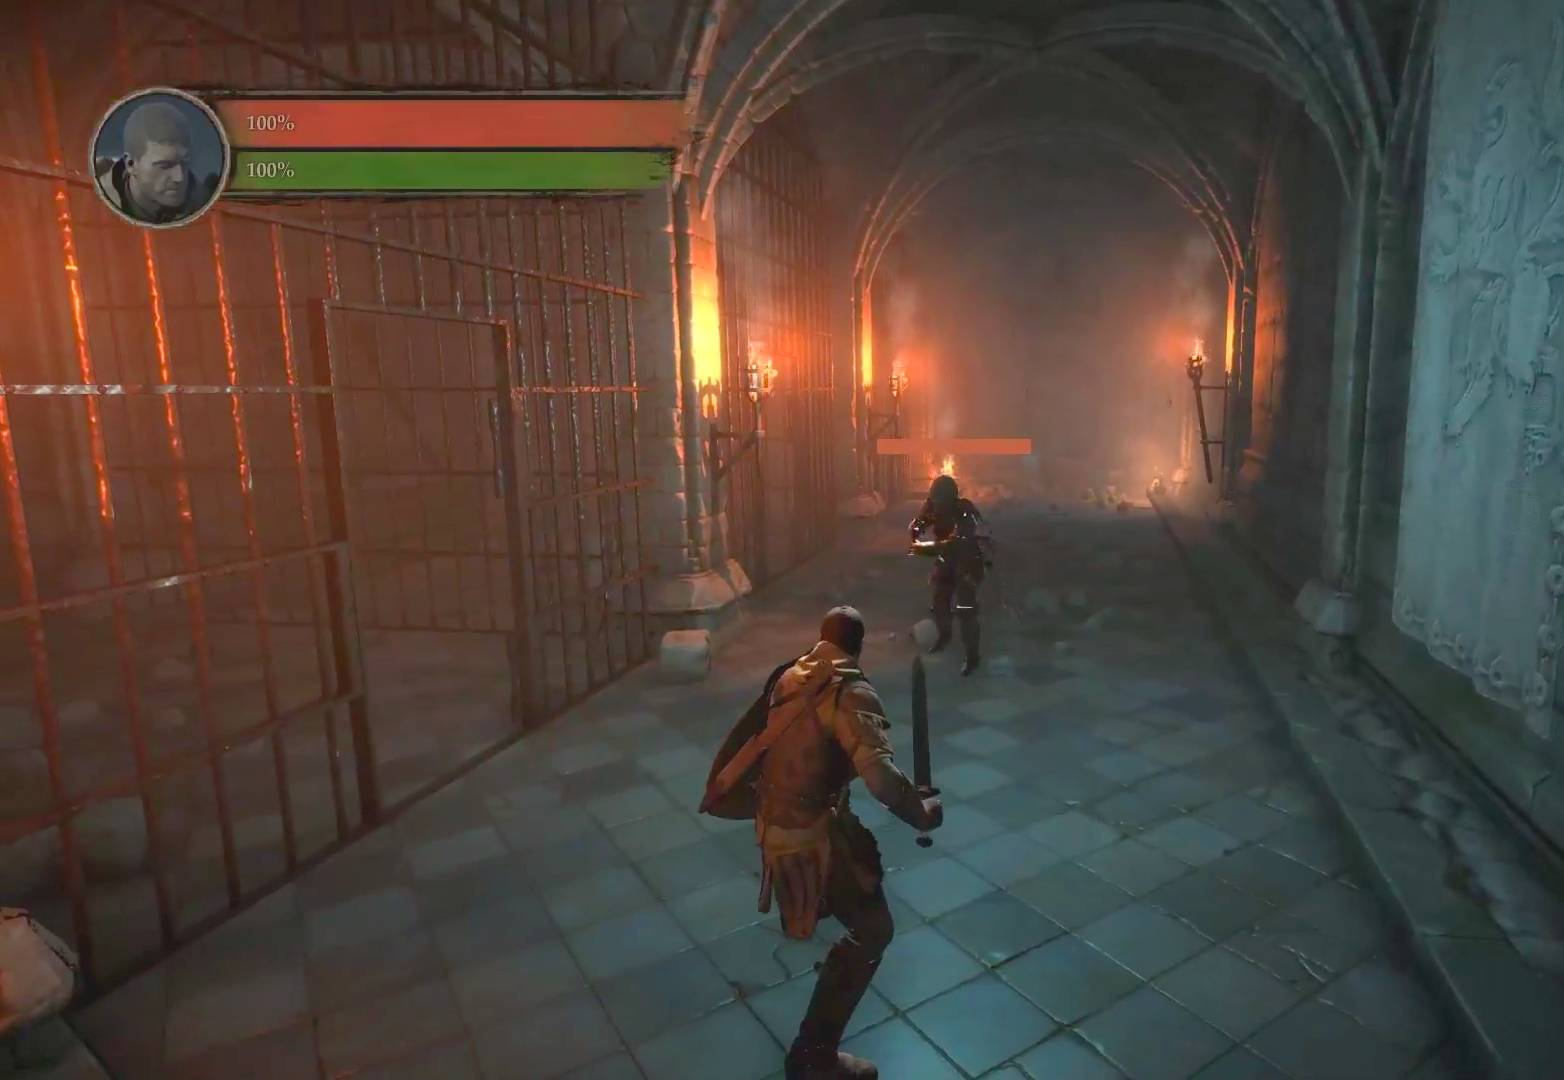
\includegraphics[width=26em]{figures/fig-bright-souls.jpg}
    \end{center}
    \legend{Source: Screen capture performed by the authors on a Microsoft Windows system.}
    \label{fig:ex1}
\end{figure}

To replicate the scenario of a successful commercial game, we look at how the problem of adaptive difficulty  is handled in multiple commercial games. Then, we analyze in depth the aspects that contribute to the difficulty of \emph{Dark Souls}, and attempt to replicate them in a simplified implementation. We compare the implementation of our solution to the original game, and outline the gameplay features that constitute the \emph{Souls}-like experience.

We propose a possible method for the design, implementation and usage of AGT as means of enhancing player experience. We compare the results in presence and absence of AGT, using as parameter a user evaluation on their perceived experience for each scenario and performance analysis based on gameplay data.